\documentclass[12pt]{report}

\usepackage[a4paper]{geometry}
%\geometry{left=2.5cm,right=2.5cm,top=2.5cm,bottom=2.5cm, a4paper}
\usepackage[utf8]{inputenc}
\usepackage{amsmath}
\usepackage{amsthm}
\usepackage{amssymb}
\usepackage{ulem}
\usepackage{graphicx}
\usepackage{caption}
\graphicspath{}
\usepackage[document]{ragged2e}
\usepackage{setspace}
\usepackage{tabularx}
\usepackage[slovene]{babel}
\usepackage{textcomp, gensymb}
\usepackage{siunitx}
\usepackage{pdfrender,xcolor}
\usepackage{hyperref}
\usepackage{xurl}
\usepackage{float}
\usepackage{titlesec}

\newfloat{slika}{htbp}{loc}
\floatname{slika}{Slika}

\newfloat{tabela}{htbp}{loc}
\floatname{tabela}{Tabela}

% Differential
\newcommand{\diff}{\mathrm{d}}

\title{
  
\includegraphics[width=0.4\textwidth]{fmf_logo}\\
  {\small Oddelek za fiziko} \\
  {Sklopljena nihajna kroga}\\
  {\small Poročilo pri fizikalnem praktikumu IV}\\

}
\date{}
\author{ Kristofer Č. Povšič \\[5 cm]
 \small  Asistentka: Jelena Vesić
}


\titleformat{\chapter}[hang]{\Huge\bfseries}{\thechapter{. }}{0pt}{\Huge\bfseries}

\setlength\parindent{0pt}

\begin{document}

\setcounter{page}{2}

\maketitle

\chapter*{Uvod}

Pri sklopitvi povzročimo, da posameznih oscilatorjev več ne obravnavamo ločeno, ampak kot en sistem. sistem sestavljen iz $n$ enakih oscilatorjev, ima $n$ lastnih nihanj, ki jih opišemo z lastnimi frekvencami $\omega_n$ in lastnimi vektorji. 

Ko povežemo dva identična nihajna kroga s kondenzatorjem $C_0$, je en način nihanja, da nihata v fazi in vmesnega sklopitvenega kondenzatorja ne zaznata. Drugi način pa je, da nihata v nasprotni fazi. 

Rešitev diferencialne enačbe za zgolj kapacitivno sklopljena kroga nam za začetni pogoj, kjer drugi krog miruje in začnemu vzbujati prvi krog, napove odvisnost napetosti oblike


\begin{align*}
  U_1 &= U_0 e^{-\beta t}\cos(\omega t) \cos (\Delta \omega t) \\ 
  U_2 &= U_0 e^{-\beta t} \cos(\omega t) \sin (\Delta \omega t)
\end{align*}


Naša eksperimentalna postavitev pa ni ravno tako idealna - predvsem je problem induktivna sklopitev, ki pri manjših vrednostih nastavljivega kondenzatorja igra precej veliko vlogo, a smo jo tu ignorirali. Ko merimo resonančno krivuljo, vidio, da je resonačni vrh položnejši, čim večje je dušenje $\beta$. Pogosto namesto parametra $\beta$ navajamo doboroto oz. kvaliteto nihajnega kroga 

\begin{equation}
  Q = \frac{\omega_1}{\Delta \omega} = \frac{\omega}{2 \beta} = \sqrt{\frac{L}{CR^2}}
\end{equation}

pri čemer je $\omega_1$ resonančna frekvenca, $\Delta \omega$ širina resonančne krivulje pri $\frac{1}{\sqrt{2}}$ maksimuma. 

\chapter*{Naloga}

\begin{itemize}
  \item Izmerite časovni potek napetosti na obeh krogih pri vzbujanju s stopničastim signalom za vse različne sklopitve $C_0 = 0,\, 150,\, 330,\, 560,\, 820,\, 1150 \si{pF}$. 
  \item Izmerite frekvenčno karakteristiko enega nihajnega kroga in določite dobroto $Q$. 
  \item Izmerite frekvenčno karakteristiko sklopljenih nihajnih krogov z meritvijo odziva drugega kroga za vsak $C_0$ in izmerite razliko lastnih krožnih frekvenc $\Delta \omega$. 
\end{itemize}


\begingroup
\let\clearpage\relax

\chapter*{Potrebščine}
\begin{itemize}
  \item digiatlni osciloskop
  \item funkcijski generator napetosti, namizni multimeter
  \item nihajna kroga in kabli, USB ključek
  \item prenosnik s programom \verb+SkNikKr+ napisan v LabView
\end{itemize}

\chapter*{Navodilo}

\begin{enumerate}
  \item Odziv obeh nihajnih krogov na napetostno stopnico: Povežem stvari kot je v navodilih in potem spreminjam sklopitveni kondenzator in opazujem signale v obeh krogih. 
  \item Vsiljeno nihanje enega nihajnega kroga: Sklopitveni kondenzator $C_0$ naj bo izklopljen, torej $C_0 = 0$ in kratko sklenimo drugi nihajni krog, tako da povežemo izhod $U_2$ in zemljo. Nato odstrani še kratko sklenitev kroga. 
  \item Vsiljeno nihanje sklopljenih krogov: Pri vklopljenem sklopitvenem kondenzatorju lahko opazimo resonančno obnašanje na obeh krogih, vendar je na drugem krogu bolj izrazito. S programom izmerite frekvenčno odvisnost od efektivne napetosti na drugem krogu v istem frekvenčnem intervalu kot pri 1. nalogi. 
\end{enumerate}

\endgroup


\chapter*{Obdelava podatkov}

\section*{1. del}

Pri različnih kapacitivnih sklopitvah posnamemo potek napetosti $U_1$ v prvem krogu, ki ga napajamo direktno in napetosti $U_2$ v krogu, ki je vzbujen. 

\begin{tabela}[H]
  \centering
  \[
    \begin{array}{|c|c|c|c|} \hline 
      C [\si{pF}] & N & Nt_0 [\pm 5 \si{\mu s}] & \omega [\pm 0.03 \mu s^{-1}]\\ \hline 
      0 & 14 & 200 & 1.26\\ 
      150 & 27 & 400 & 2.51\\
      330 & 38 & 580 & 3.64\\
      560 & 37 & 600 & 3.77\\
      820 & 37 & 635 & 3.99\\
      1150 & 36 & 630 & 3.96\\ \hline 
    \end{array}
  \]
  \caption{\small Frekvence napetosti $U_1$}
\end{tabela}

\begin{tabela}[H]
  \centering
  \[
    \begin{array}{|c|c|c|c|} \hline 
      C [\si{pF}] & N & Nt_0 [\pm 5 \si{\mu s}] & \omega [\pm 0.03 \mu s^{-1}]\\ \hline 
      0 & 22 & 310 & 1.95\\
      150 & 33 & 500 & 3.14\\
      330 & 40 & 600 & 3.77\\
      560 & 21 & 310 & 1.95\\
      820 & 21 & 340 & 2.14\\
      1150 & 30 & 500 & 3.14\\ \hline
    \end{array}
  \]
  \caption{\small Frekvence napetosti $U_2$}
\end{tabela}

\begin{tabela}
  \centering
  \[
    \begin{array}{|c|c c|c c|}\hline 
      C [\si{pF}] & \Delta \omega [\si{ms^{-1}}] & \pm [\si{ms^{-1}}] & \beta [\si{ms^{-1}}] & \pm [\si{ms^{-1}}]\\ \hline 
      0 & 31.42 &    0.79 &   10.52 &    1.04\\
      150 & 24.17 &    0.46 &    6.53 &    1.31\\
      330 & 18.48 &    0.27 &    6.12 &    1.48\\
      560 & 17.95 &    0.26 &    5.94 &    1.44\\
      820 & 16.98 &    0.23 &    5.45 &    1.37\\
      1150 & 20.27 &    0.33 &    6.28 &    1.63\\ \hline
    \end{array}
  \]
\end{tabela}

\begin{tabela}
  \centering
  \[
    \begin{array}{|c|c c|c c|}\hline 
      C [\si{pF}] & \Delta \omega [\si{ms^{-1}}] & \pm [\si{ms^{-1}}] & \beta [\si{ms^{-1}}] & \pm [\si{ms^{-1}}]\\ \hline 
      0 & 22.44 &    0.40 &    6.40 &    1.81\\
      150 & 17.70 &    0.25 &    5.68 &    1.71\\
      330 & 15.71 &    0.20 &    5.76 &    2.51\\
      560 & 23.71 &    0.45 &    6.76 &    1.92\\
      820 & 23.27 &    0.43 &    6.64 &    1.88\\
      1150 & 28.56 &    0.65 &    8.14 &    2.31\\ \hline
    \end{array}
  \]
\end{tabela}


\begin{slika}[H]
  \centering
  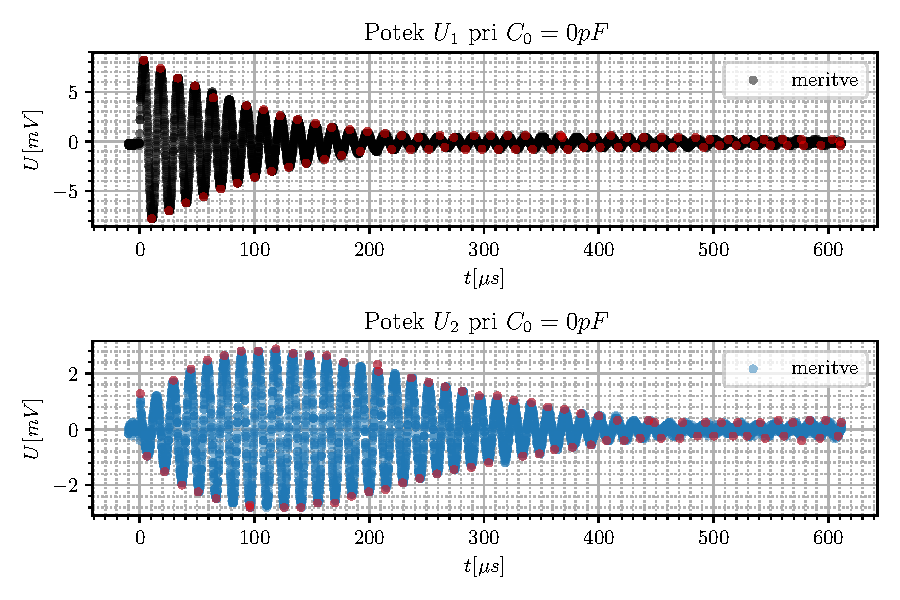
\includegraphics{C0}
  \caption{\small Poteki napetosti v prvem in drugem krogu pri $C_0 = 0\si{pF}$}
\end{slika}

\begin{slika}[H]
  \centering
  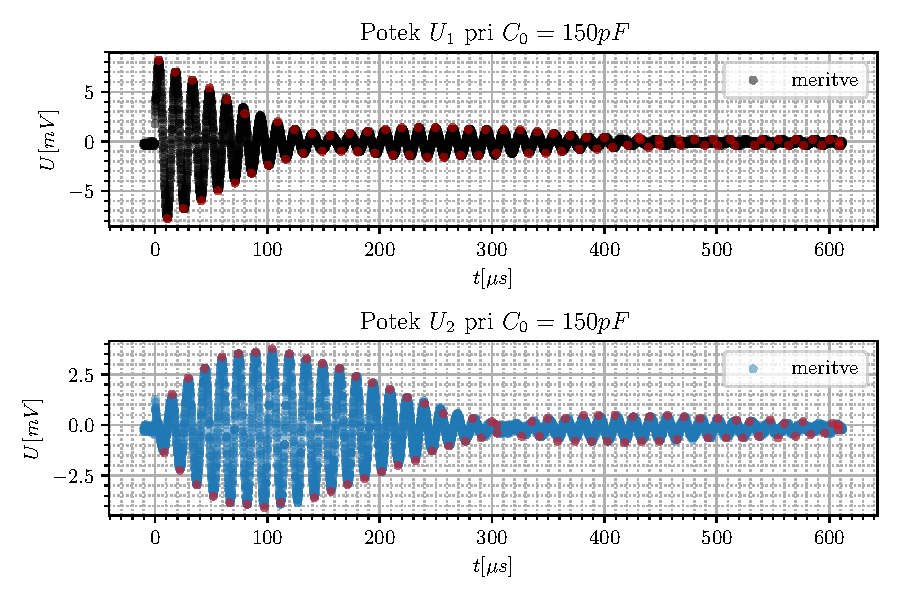
\includegraphics{C150}
  \caption{\small Poteki napetosti v prvem in drugem krogu pri $C_0 = 150\si{pF}$}
\end{slika}

\begin{slika}[H]
  \centering
  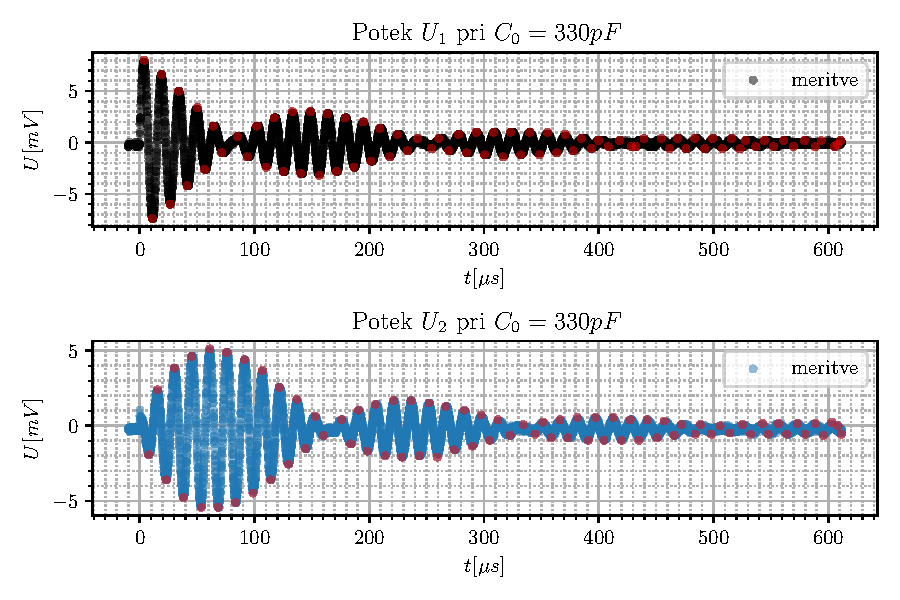
\includegraphics{C330}
  \caption{\small Poteki napetosti v prvem in drugem krogu pri $C_0 = 330\si{pF}$}
\end{slika}

\begin{slika}[H]
  \centering
  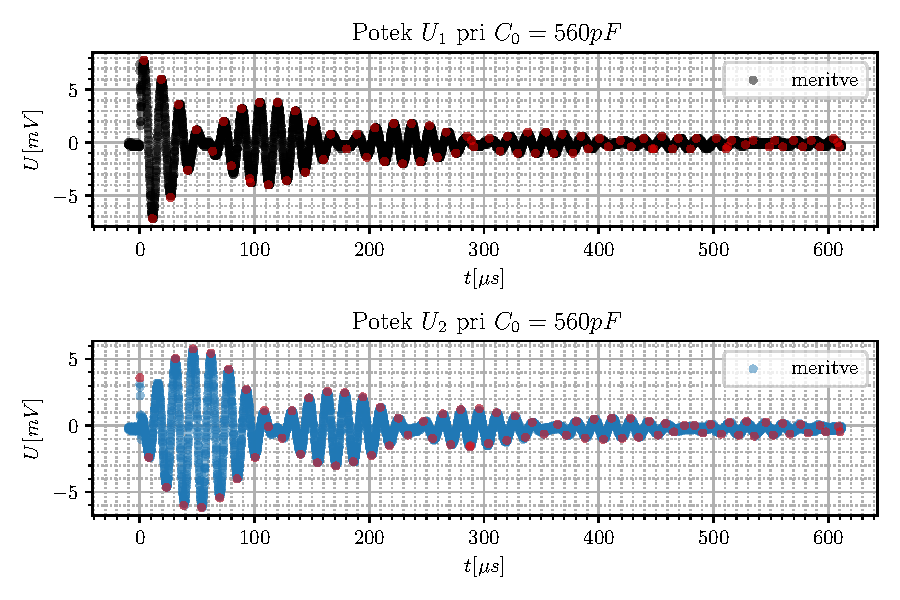
\includegraphics{C560}
  \caption{\small Poteki napetosti v prvem in drugem krogu pri $C_0 = 560\si{pF}$}
\end{slika}

\begin{slika}[H]
  \centering
  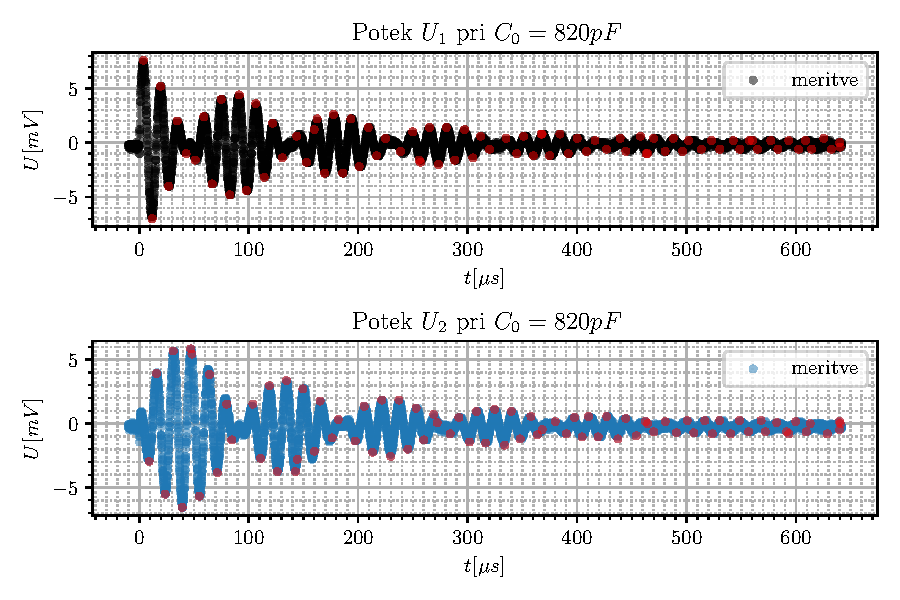
\includegraphics{C820}
  \caption{\small Poteki napetosti v prvem in drugem krogu pri $C_0 = 820\si{pF}$}
\end{slika}

\begin{slika}[H]
  \centering
  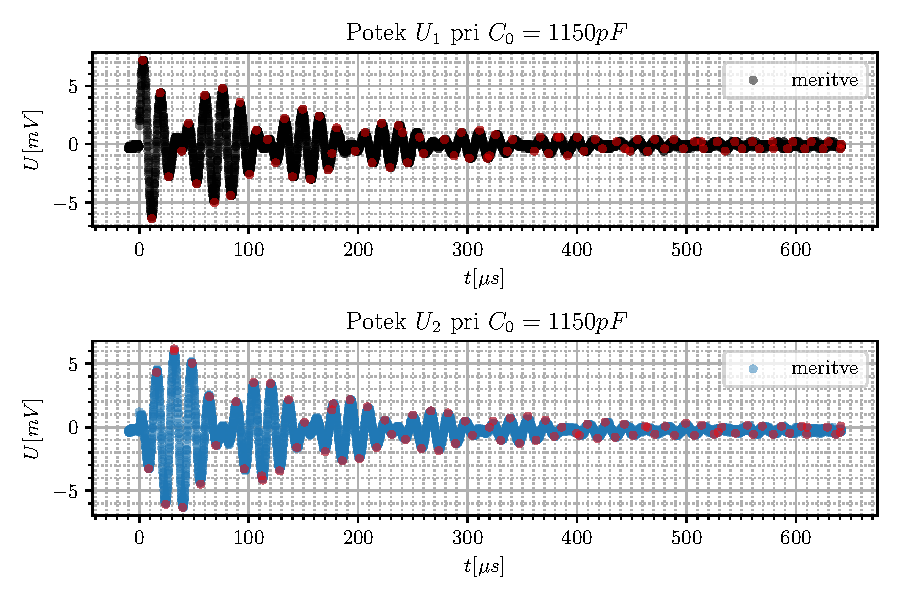
\includegraphics{C1150}
  \caption{\small Poteki napetosti v prvem in drugem krogu pri $C_0 = 1150\si{pF}$}
\end{slika}

\section*{2. del}

\begin{slika}[H]
  \centering
  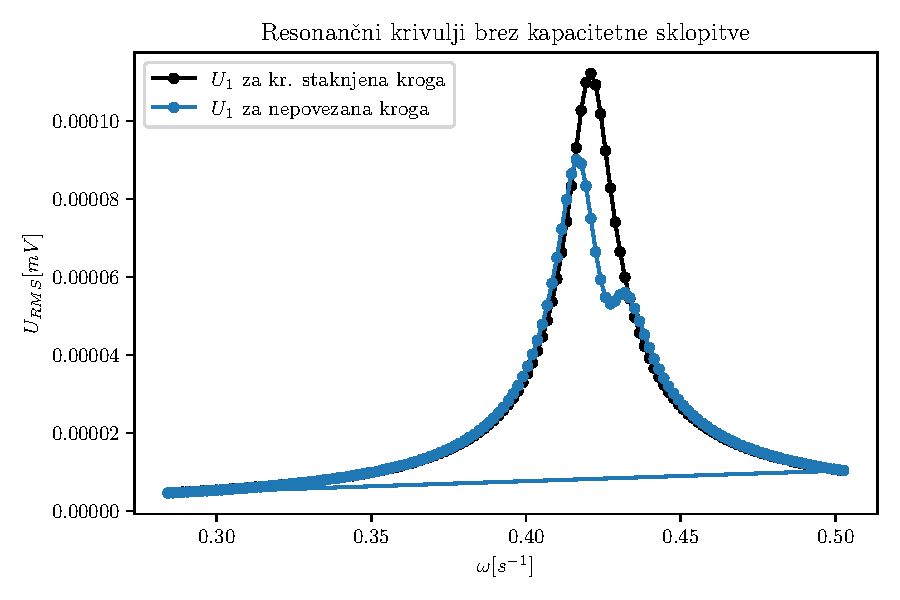
\includegraphics{vsiljenoU1}
  \caption{\small Resonančne krivulje brez sklopitve.}
\end{slika}

Izračunana dobrota je: 
\[
Q = 34 \pm 5
\]

\section*{3. del}

\begin{slika}[H]
  \centering
  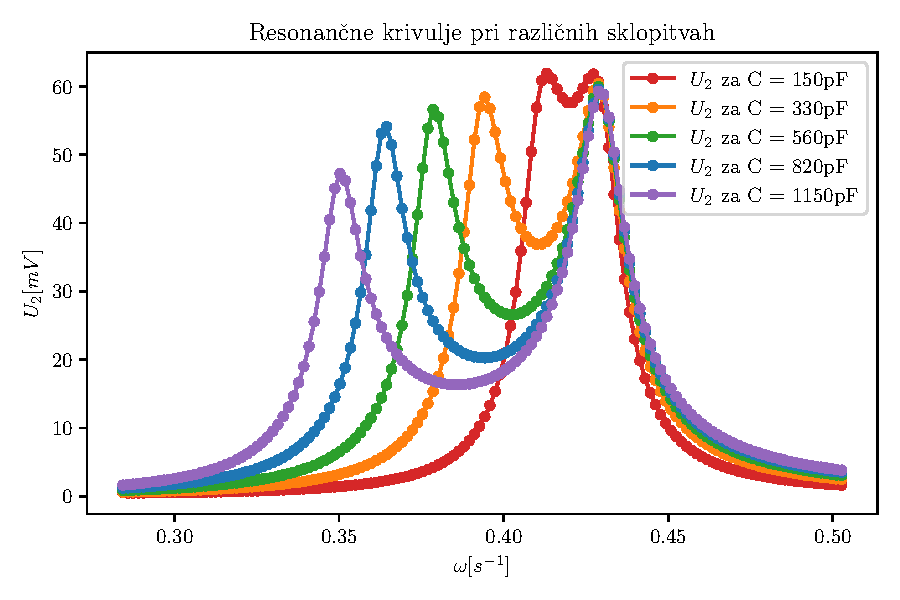
\includegraphics{vsiljenoU2}
  \caption{\small Resonančne krivulje brez sklopitve.}
\end{slika}


\begin{tabela}[H]
  \centering
  \[
    \begin{array}{|c|c|c|c|c|}\hline 
      C [\si{pF}] & \omega_1 [\si{\mu s^{-1}}] & \pm [\si{\mu s^{-1}}] & \omega_2 [\si{\mu s^{-1}}] & \pm [\si{\mu s^{-1}}]\\ \hline 
      150 & 41.3 &     0.2 &    43.0 &     0.2\\
      330 & 42.9 &     0.2 &    43.0 &     0.2\\
      560 & 42.9 &     0.2 &    43.0 &     0.2\\
      820 & 42.9 &     0.2 &    43.0 &     0.2\\
      1150 & 42.9 &     0.2 &    43.0 &     0.2\\ \hline
    \end{array}
  \]
\end{tabela}

\end{document}